\section{Method}
\label{sec:method}

Our method turns the practical question of low-NFE sampling into a calibration
problem. The input is a pretrained diffusion model, a deterministic sampler
that will be used at inference, and a desired number of steps. The output is a
schedule that spends more of those steps where the sampler's own one-step
prediction is locally unreliable. This section first defines the teacher and
student objects, then shows how teacher trajectories are used to estimate a
defect monitor and invert it into a schedule.

\subsection{Problem setup}

We start from a deterministic diffusion or flow ODE written in a
monotone sampling coordinate $u$:
\begin{equation}
  \frac{dx}{du}=f_\theta(x,u),
  \qquad u\in[u_{\min},u_{\max}].
  \label{eq:ode}
\end{equation}
The coordinate may denote time, noise level, log-SNR, or another smooth
monotone reparameterization. Let $F_{a\rightarrow b}(x)$ denote the exact
teacher flow, approximated in practice by high-accuracy numerical integration
of Eq.~\eqref{eq:ode}. If $x_0\sim p_{u_{\min}}$, the teacher marginal at
coordinate $u$ is the pushforward
\begin{equation}
  p_u=(F_{u_{\min}\rightarrow u})_{\#}p_{u_{\min}}.
  \label{eq:teacher-marginal}
\end{equation}
A fixed student solver $\mathcal S$ performs a one-step update
$\Phi_{\mathcal S}(x;u\rightarrow v)$ that approximates
$F_{u\rightarrow v}(x)$. Given a target number of steps $N$, the goal is to
construct a schedule
\begin{equation}
  U=(u_0<u_1<\cdots<u_N),\qquad
  u_0=u_{\min},\quad u_N=u_{\max},
\end{equation}
without retraining $f_\theta$ or changing the solver.

\begin{figure}[t]
  \centering
  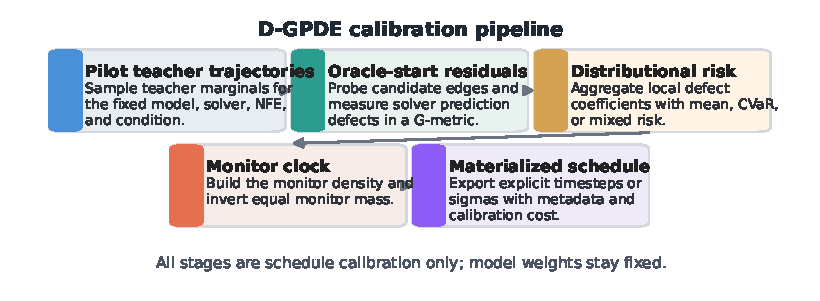
\includegraphics[width=\linewidth]{figures/dgpde_method_overview.pdf}
  \caption{Our calibration pipeline. Teacher trajectories define
  oracle-start residual probes, distributional risk forms a monitor clock, and
  equal-monitor-mass inversion materializes a solver-aware schedule. The
  schematic contains method structure only.}
  \label{fig:method-overview}
\end{figure}

\subsection{Teacher trajectories sample teacher marginals}

We draw $K$ calibration initial states $x_{k,0}\sim p_{u_{\min}}$ and compute
high-accuracy teacher trajectories
\begin{equation}
  x_k^\star(u)=F_{u_{\min}\rightarrow u}(x_{k,0}),
  \qquad k=1,\ldots,K.
\end{equation}
By Eq.~\eqref{eq:teacher-marginal}, for every coordinate $u$ the set
$\{x_k^\star(u)\}_{k=1}^K$ is a Monte Carlo sample from $p_u$. Calibration
therefore estimates a distributional object: the local state distribution on
which the student solver is evaluated.

\subsection{Geometric oracle-start defect}

We evaluate endpoint residuals with a positive definite state-space metric
$G(u)\succ0$:
\begin{equation}
  \langle r_1,r_2\rangle_{G(u)}=r_1^\top G(u)r_2,
  \qquad
  \|r\|_{G(u)}^2=r^\top G(u)r .
\end{equation}
The metric can normalize errors across noise levels, channels, or latent-space
scalings; examples include isotropic noise normalization
$G(u)=(\sigma(u)^2+\sigma_{\rm data}^2)^{-1}I$ or channel-wise whitening.

For trajectory $k$, define the $G$-unit teacher tangent
\begin{equation}
  T_{k,G}(u)
  =
  \frac{\partial_u x_k^\star(u)}
  {\|\partial_u x_k^\star(u)\|_{G(u)}}
  =
  \frac{f_\theta(x_k^\star(u),u)}
  {\|f_\theta(x_k^\star(u),u)\|_{G(u)}}.
\end{equation}
When the tangent norm is numerically unstable, we use the full residual by
setting $\rho=1$. For a residual $r$ measured at endpoint $b$, define
\begin{equation}
  \|r\|_{\rho,k,b}^2
  =
  r^\top G(b)r
  -(1-\rho)\left(T_{k,G}(b)^\top G(b)r\right)^2,
  \qquad \rho\in(0,1].
  \label{eq:mixed-norm}
\end{equation}
Equivalently, if $r=r_\parallel^{G(b)}+r_\perp^{G(b)}$ is the
$G(b)$-orthogonal tangent-normal decomposition, then
\begin{equation}
  \|r\|_{\rho,k,b}^2
  =
  \|r_\perp^{G(b)}\|_{G(b)}^2
  +
  \rho\|r_\parallel^{G(b)}\|_{G(b)}^2.
  \label{eq:mixed-decomposition}
\end{equation}
Thus $\rho=1$ gives the full residual, while $0<\rho<1$ downweights
phase-like tangent error and emphasizes normal deviation from the teacher
trajectory.

For $x\sim p_u$, the oracle-start local prediction defect of the student solver
over $[u,v]$ is
\begin{equation}
  d_{\mathcal S}(x;u,v)
  =
  \left\|
  \Phi_{\mathcal S}(x;u\rightarrow v)-F_{u\rightarrow v}(x)
  \right\|_{\rho,u,v}^{2}.
  \label{eq:oracle-defect-distribution}
\end{equation}
On calibration trajectory $k$, this becomes
\begin{equation}
  d_k(u,v)
  =
  \left\|
  \Phi_{\mathcal S}(x_k^\star(u);u\rightarrow v)-x_k^\star(v)
  \right\|_{\rho,k,v}^{2}.
  \label{eq:oracle-defect-empirical}
\end{equation}
Every measurement starts from $x_k^\star(u)$, not from a student state reached
after previous approximate steps. The defect therefore measures intrinsic
one-step solver error rather than a mixture of local defect and accumulated
prefix error.

\subsection{Local coefficient estimation and risk aggregation}

For small $h>0$, assume the local expansion
\begin{equation}
  d_{\mathcal S}(x;u,u+h)
  =
  a_{\mathcal S}(x,u)h^q+O(h^{q+1}),
  \label{eq:local-power-law-method}
\end{equation}
where $q>0$ is the effective squared-defect order and
$a_{\mathcal S}(x,u)\ge0$ is a local defect coefficient. Along trajectory $k$,
$d_k(u,u+h)=a_k(u)h^q+O(h^{q+1})$ with
$a_k(u)=a_{\mathcal S}(x_k^\star(u),u)$. Given a probe step $\eta$, a
single-probe estimate is
\begin{equation}
  \widehat a_k(u)=\frac{d_k(u,u+\eta)}{\eta^q}.
\end{equation}
When $q$ is unknown, we use multiple probe sizes $\eta_j$ and fit
\begin{equation}
  \log d_k(u,u+\eta_j)\approx \log a_k(u)+q\log\eta_j
\end{equation}
by pooled log-log regression over trajectories and probe grid points.

Let $\mathcal R$ be a risk functional over nonnegative random variables. The
distributional defect coefficient is
\begin{equation}
  \bar a_{\mathcal R}(u)
  =
  \mathcal R_{x\sim p_u}\!\left[a_{\mathcal S}(x,u)\right],
  \label{eq:distributional-a}
\end{equation}
estimated empirically by
\begin{equation}
  \widehat{\bar a}_{\mathcal R}(u)
  =
  \mathcal R_{k=1}^K\!\left[\widehat a_k(u)\right].
\end{equation}
We use mean risk, CVaR risk, or a mean-CVaR mixture:
\begin{align}
  \bar a_{\rm mean}(u)
  &=\frac{1}{K}\sum_{k=1}^K\widehat a_k(u),\\
  \bar a_{\rm CVaR}(u)
  &=\operatorname{CVaR}_{\beta,k}\!\left[\widehat a_k(u)\right],\\
  \bar a_{\alpha,\beta}(u)
  &=(1-\alpha)\bar a_{\rm mean}(u)+\alpha\bar a_{\rm CVaR}(u).
\end{align}
Mean risk targets average teacher-student alignment; CVaR emphasizes
high-error trajectories; the mixture is the default robust choice.

\subsection{Monitor clock and schedule construction}

For a small interval $[u,u+h]$, define the distributional local defect
\begin{equation}
  \bar D_{\mathcal R}(u,u+h)
  =
  \mathcal R_{x\sim p_u}\!\left[d_{\mathcal S}(x;u,u+h)\right].
\end{equation}
The local model implies
$\bar D_{\mathcal R}(u,u+h)=\bar a_{\mathcal R}(u)h^q+O(h^{q+1})$. Equalizing
the leading local risk over intervals with lengths $h_i$ requires
$\bar a_{\mathcal R}(u_i)h_i^q=C$, so the sampling density should be
proportional to $\bar a_{\mathcal R}(u)^{1/q}$. We define the monitor
\begin{equation}
  \omega_{\mathcal R}(u)
  =
  \left(\bar a_{\mathcal R}(u)+\epsilon_a\right)^{1/q},
  \label{eq:monitor}
\end{equation}
where $\epsilon_a>0$ is a numerical floor. Its interval mass is
\begin{equation}
  \mathcal M_{\mathcal R}([a,b])
  =
  \int_a^b\omega_{\mathcal R}(u)\,du.
\end{equation}
Let $\Omega_{\mathcal R}=\int_{u_{\min}}^{u_{\max}}\omega_{\mathcal R}(u)\,du$
and define the normalized monitor clock
\begin{equation}
  \tau_{\mathcal R}(u)
  =
  \frac{\int_{u_{\min}}^u\omega_{\mathcal R}(\xi)d\xi}
  {\int_{u_{\min}}^{u_{\max}}\omega_{\mathcal R}(\xi)d\xi}.
  \label{eq:monitor-clock}
\end{equation}
The final $N$-step schedule is the inverse-CDF discretization
\begin{equation}
  u_m=\tau_{\mathcal R}^{-1}\!\left(\frac{m}{N}\right),
  \qquad m=0,\ldots,N,
  \label{eq:inverse-cdf-schedule}
\end{equation}
which gives every interval equal monitor mass.

\paragraph{Calibration procedure.}
Given calibration samples, the teacher solver, target solver, metric, tangent
weight, risk functional, probe grid, probe sizes, and floor, the procedure:
\begin{enumerate}
  \item computes dense teacher trajectories $x_k^\star(u)$;
  \item evaluates oracle-start defects $d_k(u,u+\eta_j)$ on the probe grid;
  \item estimates $q$ and $a_k(u)$ from single probes or pooled log-log fits;
  \item aggregates $\widehat{\bar a}_{\mathcal R}(u)$ across trajectories;
  \item builds $\widehat\omega_{\mathcal R}(u)$, optionally smooths
  $\log\widehat\omega_{\mathcal R}$, and exports
  $u_m=\widehat\tau_{\mathcal R}^{-1}(m/N)$.
\end{enumerate}
The dominant calibration cost is $O(KMJ\,C_{\mathcal S})$, where
$M$ is the probe-grid size, $J$ is the number of probe sizes, and
$C_{\mathcal S}$ is the cost of one student probe. Changing mean aggregation to
CVaR or a mixture does not require additional model evaluations. The
implementation exports explicit timestep or sigma bundles with solver, NFE,
seed, pilot, cache, and calibration-cost metadata.
